\chapter{Desenvolvimento da Aplicação}

Neste capítulo descrevemos os conceitos, análises e ferramentas
utilizadas pela equipe TGT para o desenvolvimento do porduto Lixt,
incluindo os requisitos do projeto, as tecnologias utilizadas, e a
arquitetura e a modelagem do produto.
Isto é apresentado para que se possa estabelecer parâmetros e métricas
que guiarão o desenvolvimento e a entrega final do projeto.

\section{Arquitetura}
Com base na análise do projeto, e nos requisitos que foram levantados
como necessários, a arquitetura cliente-servidor é plausível como
modelo para o produto que pretendemos entregar.
Esta arquitetura é composta por duas aplicações distintas:
\begin{itemize}
\item Uma aplicação \emph{front-end}, focada na interação com o usúario
  e apresentação de dados de uma forma agradável e intuitiva. Esta
  aplicação será implementada em JavaScript, com o framework React
  Native, e disponibilizada para as plataformas iOS e Android.
\item Uma aplicação \emph{back-end}, que será responsável por tratar os
  dados coletados no \emph{front-end} e disponibilizar as informações
  que serão mostradas aos usuários. Como esta aplicação requer uma
  lógica de servidor, estabilidade e ampla disponiblidade, esta
  aplicação será implementada em Java, com uso do framework Spring
  Boot, que abstrai a criação de um servidor.
\end{itemize}
Podemos ver na \autoref{fig:cli-srv} uma respresentação desta
arquitetura.

\begin{figure}[h]
  \centering
  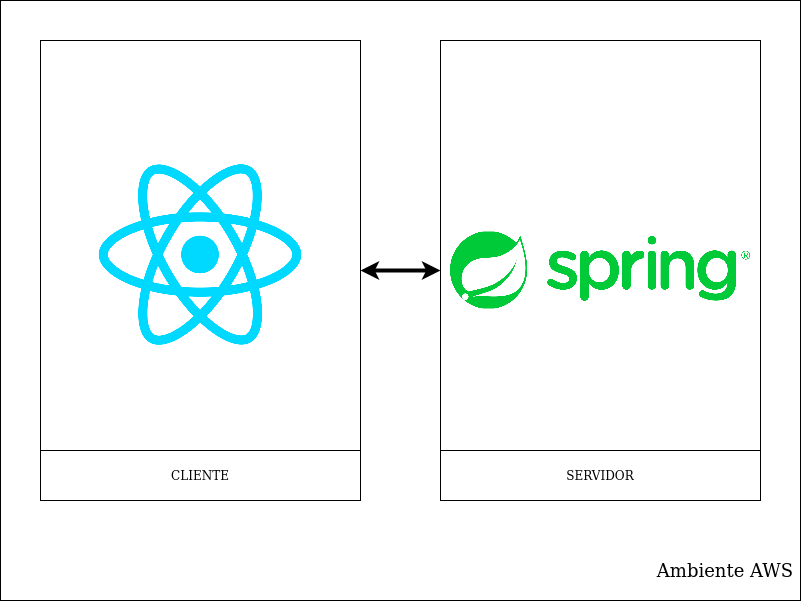
\includegraphics[scale=0.4]{lixt}
  \caption{Arquitetura Lixt}
  \label{fig:cli-srv}
\end{figure}

A comunicação entre estes serviços será feita com o uso do protocolo
\label{sig:https}\hyperlink{s:http}{HTTPS}, que permite a aplicação
cliente realizar chamadas ao servidor através de urls, seja para
buscar informações para apresentar ao usuário ou postar informações
coletadas dele. O framework Spring, além de abstrair a implementação
da lógica de um servidor, implementa \emph{listeners} para estas urls,
auxiliando a criação de pontos na aplicação do servidor focados na
comunicação com a aplicação cliente.

O uso do protocolo HTTPS oferece alguamas vantagens a aplicação
\emph{front-end}, que não precisa esperar uma solicitação ao
\emph{back-end} ser finalizada antes de realizar outras solicitações,
aumentando a repsonsividade da aplicação cliente. Para além disso,
quando combinada ao modelo \label{sig:rest}\hyperlink{s:rest}{REST} na
construção da \label{sig:API} \hyperlink{s:API}{API}, o protocolo HTTP
oferece meios eficientes para que as aplicações se comuniquem.

Como plataforma de servidor, o serviço AWS será utilizado, uma vez que
é oferecida de maneira gratuita para a realização deste projeto, e nele
serão armazenadas algumas instâncias da aplicação \emph{back-end}.
Esta redundância é necessária como forma de garantir a estabilidade do
sistema, de forma que sempre haja alguma disponível para o
processamento de novas requisições, e, em caso de falha numa delas, o
serviço não seja interrompido aos usuários.


\section{Escopo do Projeto}

Lixt é um aplicativo para gerenciamento de listas de compras compartilhadas ou não.

O aplicativo vai seguir a dinâmica de uso abaixo:
\begin{enumerate}
	\item O usuário cria uma lista de compras e insere todos os itens antes da compra;
	\item O usuário inicia um carrinho de compras quando chega ao mercado, nesse momento ele tem a opção de importar para aquele carrinho os itens das listas que ele possui em aberto (que ainda não foram finalizadas), marcando quais listas ele deseja que sejam incluídas. Com o carrinho de compras ele poderá anotar os preços dos itens, riscá-los e ver o total gasto. Ao finalizar a compra as listas são atualizadas, e já aparecem riscados os itens que já foram comprados;
	\item Quando o usuário definir que uma lista não é mais relevante ele poderá deletar a lista ou desmarcar todos os itens, para reutilizar a lista.
\end{enumerate}

A seguir listamos as principais funcionalidades como uma lista de tópicos para facilitar a visualização de quais funcionalidades dependem de outras de forma hierárquica:

\begin{itemize}
	\item \textit{Login}:
		\begin{itemize}
			\item Criar conta;
			\item Redefinir senha;
		\end{itemize}
	\item Editar uma lista:
		\begin{itemize}
			\item Adicionar item:
				\begin{itemize}
					\item Definir nome;
					\item Definir quantidade;
					\item Definir unidade de medida (un. ml, L etc.);
					\item Definir medida;
					\item Adicionar uma categoria:
						\begin{itemize}
							\item Criar nova categoria;
						\end{itemize}
					\item Adicionar um comentário;
					\item Atribuir a um usuário (caso a lista tenha sido compartilhada e pelo menos um covite já tenha sido aceito);
				\end{itemize}
			\item Remover itens;
			\item Convidar pessoas para a lista (apenas quem criou a lista):
				\begin{itemize}
					\item Enviar convite:
						\begin{itemize}
							\item Acompanhar \textit{status} (aceito ou pendente);
							\item Remover convite;
						\end{itemize}
				\end{itemize}
			\item Deletar uma lista;
			\item Limpar uma lista;
		\end{itemize}
	\item Iniciar um carrinho de compras:
		\begin{itemize}
			\item Selecionar listas para compor o carrinho;
			\item Informar o mercado onde a compra será realizada (automaticamente através da localização, se não estiver habilitada será solicitado que o usuário insira o nome do mercado);
			\item Exibir o valor total do carrinho;
			\item Informar a quantidade que será efetivamente comprada naquele momento (o usuário pode ter planejado 10 unidades e apenas comprar 5 naquele momento);
			\item Riscar itens;
			\item Finalizar um carrinho de compras;
		\end{itemize}
	\item Ver estatísticas:
		\begin{itemize}
			\item Selecionar uma lista e ver o total gasto naquela lista ao longo do tempo em um gráfico de linha:
				\begin{itemize}
					\item Selecionar um dos pontos do gráfico e ver detalhes daquela lista;
				\end{itemize}
			\item Selecionar uma lista para ver um gráfico de pizza com os valores médios gastos por categorias naquela lista;
			\item Verificar histórico de preços de um item (tabela com nome do produto, quantidade, marca, preço, mercado e data da compra):
				\begin{itemize}
					\item Selecionar uma lista, dentro da lista selecionada selecionar o produto para ver o histórico;
				\end{itemize}
		\end{itemize}
\end{itemize}

Para o \textit{Minimum Viable Product} (\label{sig:mvp}\hyperlink{s:mvp}{MVP}) vamos implementar as seguintes funcionalidades, as demais ficarão para o próximo semestre:

\begin{itemize}
	\item \textit{Login}:
		\begin{itemize}
			\item Criar conta;
			\item Redefinir senha;
		\end{itemize}
	\item Criar lista de compra:
		\begin{itemize}
			\item Atribuir um nome;
			\item Atribuir uma descrição;
			\item Importar uma lista anterior;
		\end{itemize}
	\item Editar uma lista:
		\begin{itemize}
			\item Adicionar item:
				\begin{itemize}
					\item Definir nome;
					\item Definir quantidade;
					\item Definir unidade de medida (un., ml., L etc);
					\item Definir medida;
					\item Adicionar a uma categoria:
						\begin{itemize}
							\item Criar uma nova categoria;
						\end{itemize}
					\item Adicionar um comentário;
					\item Atribuir a um usuário (caso a lista tenha sido compartilhada e pelo menos um covite já tenha sido aceito);
				\end{itemize}
			\item Remover itens;
			\item Convidar pessoas para a lista (apenas quem criou a lista):
				\begin{itemize}
					\item Enviar convite:
						\begin{itemize}
							\item Acompanhar  status (aceito ou pendente);
							\item Remover convite;
						\end{itemize}
				\end{itemize}
			\item Deletar uma lista;
			\item Limpar uma lista;
		\end{itemize}
	\item Iniciar um carrinho de compras:
		\begin{itemize}
			\item Selecionar listas para compor o carrinho;
			\item Informar o mercado onde a compra será realizada (será solicitado que o usuário insira o nome do mercado manualmente);
			\item Exibir o valor total do carrinho;
			\item Informar a quantidade que será efetivamente comprada naquele momento (o usuário pode ter planejado 10 unidades e apenas comprar 5 naquele momento);
			\item Riscar itens;
			\item Finalizar o carrinho de compras.
		\end{itemize}
\end{itemize}

\subsubsection{Requisitos Funcionais}

Os requisitos funcionais dizem respeito às funcionalidade que o sistema deve ter. A Tabela \ref{reqFuncionais} lista os requisitos funcionais, suas dependências, a sigla e a prioridade de implementação.

\begin{table}[H]
\caption{Requisitos funcionais}
\begin{tabular}{|l|l|l|l|l}
\cline{1-4}
\textbf{Sigla} & \textbf{Descrição}                                                                                                                                                                                                                                               & \textbf{Prioridade} & \textbf{Dependências} &  \\ \cline{1-4}
RF01           & \begin{tabular}[c]{@{}l@{}}\textit{Login}: o usuário deve ser capaz de criar \\ sua conta no aplicativo, definir sua senha e \\ realizar o \textit{login} no sistema.\end{tabular}                                                                                                 & Alta                &                       &  \\ \cline{1-4}
RF02           & \begin{tabular}[c]{@{}l@{}}O sistema deve possibilitar que o usuário \\ crie suas listas de compras e possa atribuir um\\ nome, uma descrição e ter a opção de importar \\ uma lista existente.\end{tabular}                                                     & Alta                & RF01                  &  \\ \cline{1-4}
RF03           & \begin{tabular}[c]{@{}l@{}}Editar uma lista: Possibilita ao usuário o \\ gerenciamento dos itens da lista, como adicionar \\ itens, remover e enviar convites para a lista.\end{tabular}                                                                         & Alta                & RF02                  &  \\ \cline{1-4}
RF04           & \begin{tabular}[c]{@{}l@{}}Iniciar um carrinho de compras: permitir que o \\ usuário importe várias listas de compras, informe \\ o local da compra, o total gasto, quantidade de \\ itens a ser comprados, riscar itens e finalizar \\ o carrinho.\end{tabular} & Alta                & RF03                  &  \\ \cline{1-4}
RF05           & \begin{tabular}[c]{@{}l@{}}Ver estatísticas: ver o histórico de valores \\ pagos em uma lista ao longo do tempo, ver \\ os valores gastos por categorias em uma lista, \\ ver o histórico de preços de um determinado \\ item ao longo do tempo.\end{tabular}    & Média               & RF04                  &  \\ \cline{1-4}
\end{tabular}
\fonte{Os Autores}
\label{reqFuncionais}
\end{table}


\subsubsection{Requisitos Não Funcionais}

De maneira simplificada, os requisitos não funcionais não estão relacionados diretamente às funcionalidades do sistema, mas ao seu funcionamento de um modo geral, ou seja, como ele as funcionalidade serão executadas.

Na Tabela \ref{reqNaoFuncionais} estão elencados os requisitos não funcionais, cada um com sua nomenclatura, categoria e descrição.

\begin{table}[H]
\caption{Requisitos Não funcionais}
\begin{tabular}{llll}
\cline{1-3}
\multicolumn{1}{|l|}{\textbf{Nomenclatura}} & \multicolumn{1}{l|}{\textbf{Descrição}}                                                                                                                                                                                                            & \multicolumn{1}{l|}{\textbf{Categoria}} &  \\ \cline{1-3}
\multicolumn{1}{|l|}{RNF01}                 & \multicolumn{1}{l|}{\begin{tabular}[c]{@{}l@{}}Criptografia das senhas: Por uma questão \\ de segurança as senhas não serão \\ armazenadas diretamente no banco, serão \\ criptografadas antes de serem armazenadas \\ como um \textit{hash}.\end{tabular}} & \multicolumn{1}{l|}{Segurança}          &  \\ \cline{1-3}
\multicolumn{1}{|l|}{RNF02}                 & \multicolumn{1}{l|}{\begin{tabular}[c]{@{}l@{}}Comunicação: A comunicação entre as \\ camadas da aplicação deverá ser feita utilizando \\ o protocolo HTTPS, para garantir a segurança \\ no envio dos dados através da rede.\end{tabular}}        & \multicolumn{1}{l|}{Segurança}          &  \\ \cline{1-3}
\multicolumn{1}{|l|}{RNF03}                 & \multicolumn{1}{l|}{\begin{tabular}[c]{@{}l@{}}Responsividade: O sistema deve exibir \\ corretamente os elementos da interface gráfica \\ nos mais variados tamanhos de celulares.\end{tabular}}                                                   & \multicolumn{1}{l|}{Usabilidade}        &  \\ \cline{1-3}
\multicolumn{1}{|l|}{RNF04}                 & \multicolumn{1}{l|}{\begin{tabular}[c]{@{}l@{}}Internacionalização: O sistema deverá suportar \\ dois idiomas (inglês e português) e suportar \\ que futuramente seja possível adicionar outros \\ idiomas.\end{tabular}}                          & \multicolumn{1}{l|}{Usabilidade}        &  \\ \cline{1-3}
\multicolumn{1}{|l|}{RNF05}                 & \multicolumn{1}{l|}{\begin{tabular}[c]{@{}l@{}}Escalabilidade: O sistema deverá ser projetado \\ para garantir que futuras melhoras e expansões \\ sejam possíveis.\end{tabular}}                                                                  & \multicolumn{1}{l|}{Desempenho}         &  \\ \cline{1-3}
\multicolumn{1}{|l|}{RNF06}                 & \multicolumn{1}{l|}{\begin{tabular}[c]{@{}l@{}}Disponibilidade: O sistema deverá estar disponível \\ aos usuários ininterruptamente\end{tabular}}                                                                                                  & \multicolumn{1}{l|}{Disponibilidade}    &  \\ \cline{1-3}
                                            &                                                                                                                                                                                                                                                    &                                         & 
\end{tabular}
\label{reqNaoFuncionais}
\fonte{Os Autores}
\end{table}


\section{Segurança, Privacidade e Legislação}

A principal lei brasileira que trata de tratamento de dados  nos meios digitais é a lei N° 13.709, sancionada em 14 de Agosto de 2018 \cite{leigpd} e que entrou em vigor no ano de 2020, conhecida como Lei Geral de Proteção de Dados (\label{sig:lgpd}\hyperlink{s:lgpd}{LGPD}).

Seguindo o disposto no Artigo 6°, inciso terceiro da LGPD, a aplicação vai coletar o mínimo de dados do usuário necessários para uso da aplicação, os dados serão: localização, endereço de email e nome do usuário. Sendo facultativo ao usuário ativar ou não a sua localização.

O design da aplicação vai seguir o princípio da transparência. O usuário do aplicativo será informado de quais as informações que serão coletadas. O próprio sistema Android, por padrão, solicita ao usuário permissão para uso da localização, um dos dados que será necessário coletar, caso o usuário opte pela detecção do local da compra automaticamente.

Como a maioria dos sistemas atuais, utilizaremos uma API (Application Program Interface) para realizar a comunicação e transferência de dados entre a interface de usuário e o servidor. Essa arquitetura possui intrinsecamente vulnerabilidades conhecidas e quando não são bem projetadas as API’s podem ser um dos pontos fracos do sistema quando se trata de segurança. A empresa de consultoria Gartner \cite{anilLamba} prevê que a tendência é que em 2022 as API’s se tornem o principal foco de ataques cibernéticos.

Cientes desse cenário, foi definido que o sistema deverá seguir algumas boas práticas de desenvolvimento, citadas brevemente a seguir:
\begin{itemize}
	\item Autenticação: As requisições apenas serão aceitas se o usuário estiver logado no sistema;
	\item Criptografia: Para evitar ataques do tipo man-in-the-middle as mensagens entre cliente e servidor serão criptografadas, seguindo o protocolo HTTPS;
	\item Documentação dos \textit{endpoints} sensíveis: Será feito um levantamento de todos os \textit{endpoints} que acessam informações sensíveis, para garantir que apenas usuários autenticados tenham acesso;
\end{itemize}

Como medida de segurança, o banco de dados não irá armazenar as senhas das contas dos usuários e sim um \textit{hash} da senha, e este será comparado com o \textit{hash} da senha informado no momento do login. Ainda como uma forma de segurança, ao cadastrar a senha ou mudar a senha atual o usuário não poderá cadastrar senha que não possua menos de seis dígitos, e que não tenham letras maiúsculas e minúsculas e números, e deverá ter no mínimo um caractere especial.

%%% Local Variables:
%%% mode: latex
%%% TeX-master: "../desenho"
%%% End:
